% Created by tikzDevice version 0.12.6 on 2025-05-06 22:53:29
% !TEX encoding = UTF-8 Unicode
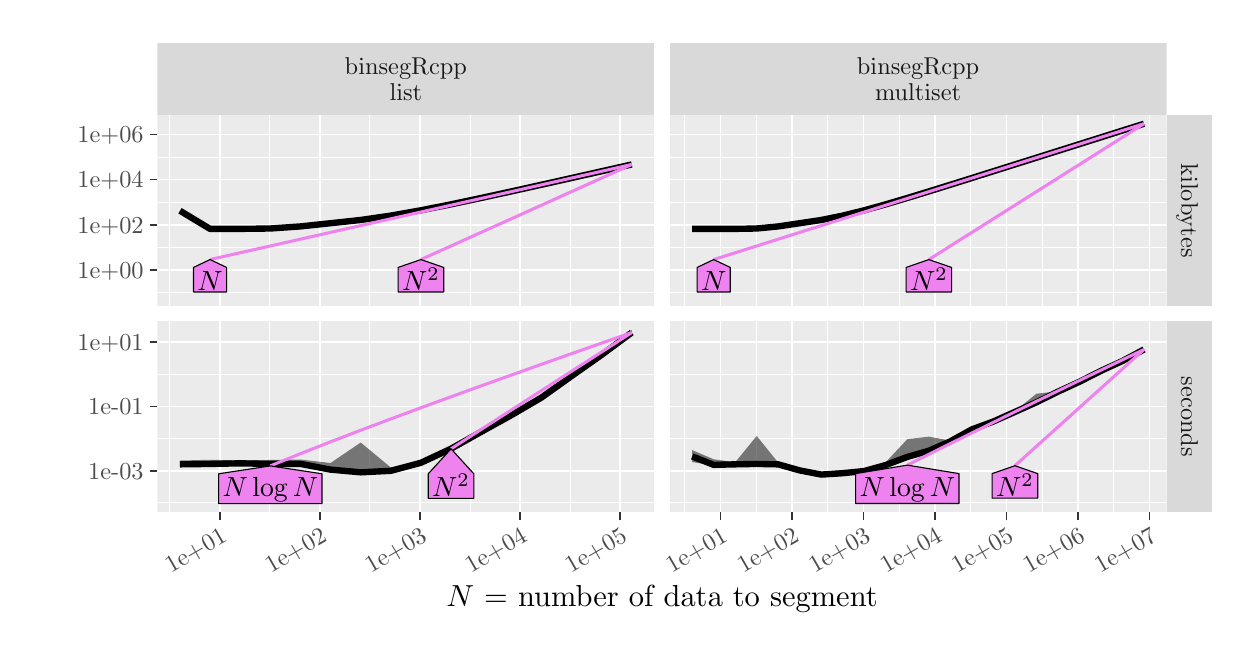
\begin{tikzpicture}[x=1pt,y=1pt]
\definecolor{fillColor}{RGB}{255,255,255}
\path[use as bounding box,fill=fillColor,fill opacity=0.00] (0,0) rectangle (433.62,216.81);
\begin{scope}
\path[clip] (  0.00,  0.00) rectangle (433.62,216.81);
\definecolor{drawColor}{RGB}{255,255,255}
\definecolor{fillColor}{RGB}{255,255,255}

\path[draw=drawColor,line width= 0.6pt,line join=round,line cap=round,fill=fillColor] ( -0.00,  0.00) rectangle (433.62,216.81);
\end{scope}
\begin{scope}
\path[clip] ( 46.86,116.18) rectangle (226.46,185.23);
\definecolor{fillColor}{gray}{0.92}

\path[fill=fillColor] ( 46.86,116.18) rectangle (226.46,185.23);
\definecolor{drawColor}{RGB}{255,255,255}

\path[draw=drawColor,line width= 0.3pt,line join=round] ( 46.86,121.16) --
	(226.46,121.16);

\path[draw=drawColor,line width= 0.3pt,line join=round] ( 46.86,137.47) --
	(226.46,137.47);

\path[draw=drawColor,line width= 0.3pt,line join=round] ( 46.86,153.77) --
	(226.46,153.77);

\path[draw=drawColor,line width= 0.3pt,line join=round] ( 46.86,170.08) --
	(226.46,170.08);

\path[draw=drawColor,line width= 0.3pt,line join=round] ( 51.34,116.18) --
	( 51.34,185.23);

\path[draw=drawColor,line width= 0.3pt,line join=round] ( 87.49,116.18) --
	( 87.49,185.23);

\path[draw=drawColor,line width= 0.3pt,line join=round] (123.65,116.18) --
	(123.65,185.23);

\path[draw=drawColor,line width= 0.3pt,line join=round] (159.81,116.18) --
	(159.81,185.23);

\path[draw=drawColor,line width= 0.3pt,line join=round] (195.97,116.18) --
	(195.97,185.23);

\path[draw=drawColor,line width= 0.6pt,line join=round] ( 46.86,129.31) --
	(226.46,129.31);

\path[draw=drawColor,line width= 0.6pt,line join=round] ( 46.86,145.62) --
	(226.46,145.62);

\path[draw=drawColor,line width= 0.6pt,line join=round] ( 46.86,161.92) --
	(226.46,161.92);

\path[draw=drawColor,line width= 0.6pt,line join=round] ( 46.86,178.23) --
	(226.46,178.23);

\path[draw=drawColor,line width= 0.6pt,line join=round] ( 69.42,116.18) --
	( 69.42,185.23);

\path[draw=drawColor,line width= 0.6pt,line join=round] (105.57,116.18) --
	(105.57,185.23);

\path[draw=drawColor,line width= 0.6pt,line join=round] (141.73,116.18) --
	(141.73,185.23);

\path[draw=drawColor,line width= 0.6pt,line join=round] (177.89,116.18) --
	(177.89,185.23);

\path[draw=drawColor,line width= 0.6pt,line join=round] (214.04,116.18) --
	(214.04,185.23);
\definecolor{drawColor}{RGB}{0,0,0}

\path[draw=drawColor,line width= 2.3pt,line join=round] ( 55.03,150.65) --
	( 65.91,144.09) --
	( 76.80,144.10) --
	( 87.68,144.24) --
	( 98.56,144.99) --
	(109.45,146.15) --
	(120.33,147.32) --
	(131.22,148.90) --
	(142.10,150.82) --
	(152.99,152.98) --
	(163.87,155.27) --
	(174.76,157.64) --
	(185.64,160.05) --
	(196.52,162.48) --
	(207.41,164.93) --
	(218.29,167.38);
\definecolor{drawColor}{RGB}{238,130,238}

\path[draw=drawColor,line width= 1.1pt,line join=round] (142.10,133.02) --
	(152.99,137.93) --
	(163.87,142.84) --
	(174.76,147.74) --
	(185.64,152.65) --
	(196.52,157.56) --
	(207.41,162.47) --
	(218.29,167.38);

\path[draw=drawColor,line width= 1.1pt,line join=round] ( 65.91,133.02) --
	( 76.80,135.47) --
	( 87.68,137.93) --
	( 98.56,140.38) --
	(109.45,142.84) --
	(120.33,145.29) --
	(131.22,147.74) --
	(142.10,150.20) --
	(152.99,152.65) --
	(163.87,155.11) --
	(174.76,157.56) --
	(185.64,160.01) --
	(196.52,162.47) --
	(207.41,164.92) --
	(218.29,167.38);
\end{scope}
\begin{scope}
\path[clip] ( 46.86,116.18) rectangle (226.46,185.23);
\definecolor{drawColor}{RGB}{0,0,0}
\definecolor{fillColor}{RGB}{238,130,238}

\path[draw=drawColor,line width= 0.4pt,line join=round,line cap=round,fill=fillColor] (133.87,130.17) --
	(142.10,133.02) --
	(150.33,130.17) --
	(150.33,121.31) --
	(133.87,121.31) --
	cycle;

\path[draw=drawColor,line width= 0.4pt,line join=round,line cap=round,fill=fillColor] ( 59.93,130.17) --
	( 65.91,133.02) --
	( 71.90,130.17) --
	( 71.90,121.31) --
	( 59.93,121.31) --
	cycle;

\node[text=drawColor,anchor=base,inner sep=0pt, outer sep=0pt, scale=  1.00] at (142.10,121.86) {$N^2$};

\node[text=drawColor,anchor=base,inner sep=0pt, outer sep=0pt, scale=  1.00] at ( 65.91,121.86) {$N$};
\end{scope}
\begin{scope}
\path[clip] ( 46.86, 41.62) rectangle (226.46,110.68);
\definecolor{fillColor}{gray}{0.92}

\path[fill=fillColor] ( 46.86, 41.62) rectangle (226.46,110.68);
\definecolor{drawColor}{RGB}{255,255,255}

\path[draw=drawColor,line width= 0.3pt,line join=round] ( 46.86, 45.09) --
	(226.46, 45.09);

\path[draw=drawColor,line width= 0.3pt,line join=round] ( 46.86, 68.35) --
	(226.46, 68.35);

\path[draw=drawColor,line width= 0.3pt,line join=round] ( 46.86, 91.60) --
	(226.46, 91.60);

\path[draw=drawColor,line width= 0.3pt,line join=round] ( 51.34, 41.62) --
	( 51.34,110.68);

\path[draw=drawColor,line width= 0.3pt,line join=round] ( 87.49, 41.62) --
	( 87.49,110.68);

\path[draw=drawColor,line width= 0.3pt,line join=round] (123.65, 41.62) --
	(123.65,110.68);

\path[draw=drawColor,line width= 0.3pt,line join=round] (159.81, 41.62) --
	(159.81,110.68);

\path[draw=drawColor,line width= 0.3pt,line join=round] (195.97, 41.62) --
	(195.97,110.68);

\path[draw=drawColor,line width= 0.6pt,line join=round] ( 46.86, 56.72) --
	(226.46, 56.72);

\path[draw=drawColor,line width= 0.6pt,line join=round] ( 46.86, 79.97) --
	(226.46, 79.97);

\path[draw=drawColor,line width= 0.6pt,line join=round] ( 46.86,103.23) --
	(226.46,103.23);

\path[draw=drawColor,line width= 0.6pt,line join=round] ( 69.42, 41.62) --
	( 69.42,110.68);

\path[draw=drawColor,line width= 0.6pt,line join=round] (105.57, 41.62) --
	(105.57,110.68);

\path[draw=drawColor,line width= 0.6pt,line join=round] (141.73, 41.62) --
	(141.73,110.68);

\path[draw=drawColor,line width= 0.6pt,line join=round] (177.89, 41.62) --
	(177.89,110.68);

\path[draw=drawColor,line width= 0.6pt,line join=round] (214.04, 41.62) --
	(214.04,110.68);
\definecolor{fillColor}{RGB}{0,0,0}

\path[fill=fillColor,fill opacity=0.50] ( 55.03, 60.40) --
	( 65.91, 60.67) --
	( 76.80, 60.43) --
	( 87.68, 60.60) --
	( 98.56, 60.76) --
	(109.45, 59.50) --
	(120.33, 66.90) --
	(131.22, 57.88) --
	(142.10, 60.23) --
	(152.99, 64.81) --
	(163.87, 70.91) --
	(174.76, 76.91) --
	(185.64, 83.30) --
	(196.52, 91.03) --
	(207.41, 98.65) --
	(218.29,107.54) --
	(218.29,106.55) --
	(207.41, 98.54) --
	(196.52, 90.85) --
	(185.64, 82.89) --
	(174.76, 76.69) --
	(163.87, 70.67) --
	(152.99, 64.48) --
	(142.10, 58.99) --
	(131.22, 56.22) --
	(120.33, 55.43) --
	(109.45, 56.30) --
	( 98.56, 58.85) --
	( 87.68, 58.94) --
	( 76.80, 59.07) --
	( 65.91, 58.74) --
	( 55.03, 58.77) --
	cycle;

\path[] ( 55.03, 60.40) --
	( 65.91, 60.67) --
	( 76.80, 60.43) --
	( 87.68, 60.60) --
	( 98.56, 60.76) --
	(109.45, 59.50) --
	(120.33, 66.90) --
	(131.22, 57.88) --
	(142.10, 60.23) --
	(152.99, 64.81) --
	(163.87, 70.91) --
	(174.76, 76.91) --
	(185.64, 83.30) --
	(196.52, 91.03) --
	(207.41, 98.65) --
	(218.29,107.54);

\path[] (218.29,106.55) --
	(207.41, 98.54) --
	(196.52, 90.85) --
	(185.64, 82.89) --
	(174.76, 76.69) --
	(163.87, 70.67) --
	(152.99, 64.48) --
	(142.10, 58.99) --
	(131.22, 56.22) --
	(120.33, 55.43) --
	(109.45, 56.30) --
	( 98.56, 58.85) --
	( 87.68, 58.94) --
	( 76.80, 59.07) --
	( 65.91, 58.74) --
	( 55.03, 58.77);
\definecolor{drawColor}{RGB}{0,0,0}

\path[draw=drawColor,line width= 2.3pt,line join=round] ( 55.03, 59.02) --
	( 65.91, 59.16) --
	( 76.80, 59.39) --
	( 87.68, 59.17) --
	( 98.56, 59.18) --
	(109.45, 57.11) --
	(120.33, 56.13) --
	(131.22, 56.68) --
	(142.10, 59.59) --
	(152.99, 64.67) --
	(163.87, 70.76) --
	(174.76, 76.78) --
	(185.64, 83.14) --
	(196.52, 90.91) --
	(207.41, 98.58) --
	(218.29,106.64);
\definecolor{drawColor}{RGB}{238,130,238}

\path[draw=drawColor,line width= 1.1pt,line join=round] ( 87.68, 58.45) --
	( 98.56, 62.87) --
	(109.45, 67.15) --
	(120.33, 71.33) --
	(131.22, 75.42) --
	(142.10, 79.46) --
	(152.99, 83.44) --
	(163.87, 87.38) --
	(174.76, 91.28) --
	(185.64, 95.16) --
	(196.52, 99.01) --
	(207.41,102.83) --
	(218.29,106.64);

\path[draw=drawColor,line width= 1.1pt,line join=round] (152.99, 64.63) --
	(163.87, 71.63) --
	(174.76, 78.64) --
	(185.64, 85.64) --
	(196.52, 92.64) --
	(207.41, 99.64) --
	(218.29,106.64);
\end{scope}
\begin{scope}
\path[clip] ( 46.86, 41.62) rectangle (226.46,110.68);
\definecolor{drawColor}{RGB}{0,0,0}
\definecolor{fillColor}{RGB}{238,130,238}

\path[draw=drawColor,line width= 0.4pt,line join=round,line cap=round,fill=fillColor] ( 69.01, 55.61) --
	( 87.68, 58.45) --
	(106.35, 55.61) --
	(106.35, 44.80) --
	( 69.01, 44.80) --
	cycle;

\path[draw=drawColor,line width= 0.4pt,line join=round,line cap=round,fill=fillColor] (144.76, 55.61) --
	(152.99, 64.63) --
	(161.21, 55.61) --
	(161.21, 46.74) --
	(144.76, 46.74) --
	cycle;

\node[text=drawColor,anchor=base,inner sep=0pt, outer sep=0pt, scale=  1.00] at ( 87.68, 47.30) {$N \log N$};

\node[text=drawColor,anchor=base,inner sep=0pt, outer sep=0pt, scale=  1.00] at (152.99, 47.30) {$N^2$};
\end{scope}
\begin{scope}
\path[clip] (231.96,116.18) rectangle (411.55,185.23);
\definecolor{fillColor}{gray}{0.92}

\path[fill=fillColor] (231.96,116.18) rectangle (411.55,185.23);
\definecolor{drawColor}{RGB}{255,255,255}

\path[draw=drawColor,line width= 0.3pt,line join=round] (231.96,121.16) --
	(411.55,121.16);

\path[draw=drawColor,line width= 0.3pt,line join=round] (231.96,137.47) --
	(411.55,137.47);

\path[draw=drawColor,line width= 0.3pt,line join=round] (231.96,153.77) --
	(411.55,153.77);

\path[draw=drawColor,line width= 0.3pt,line join=round] (231.96,170.08) --
	(411.55,170.08);

\path[draw=drawColor,line width= 0.3pt,line join=round] (237.48,116.18) --
	(237.48,185.23);

\path[draw=drawColor,line width= 0.3pt,line join=round] (263.31,116.18) --
	(263.31,185.23);

\path[draw=drawColor,line width= 0.3pt,line join=round] (289.14,116.18) --
	(289.14,185.23);

\path[draw=drawColor,line width= 0.3pt,line join=round] (314.96,116.18) --
	(314.96,185.23);

\path[draw=drawColor,line width= 0.3pt,line join=round] (340.79,116.18) --
	(340.79,185.23);

\path[draw=drawColor,line width= 0.3pt,line join=round] (366.62,116.18) --
	(366.62,185.23);

\path[draw=drawColor,line width= 0.3pt,line join=round] (392.44,116.18) --
	(392.44,185.23);

\path[draw=drawColor,line width= 0.6pt,line join=round] (231.96,129.31) --
	(411.55,129.31);

\path[draw=drawColor,line width= 0.6pt,line join=round] (231.96,145.62) --
	(411.55,145.62);

\path[draw=drawColor,line width= 0.6pt,line join=round] (231.96,161.92) --
	(411.55,161.92);

\path[draw=drawColor,line width= 0.6pt,line join=round] (231.96,178.23) --
	(411.55,178.23);

\path[draw=drawColor,line width= 0.6pt,line join=round] (250.40,116.18) --
	(250.40,185.23);

\path[draw=drawColor,line width= 0.6pt,line join=round] (276.22,116.18) --
	(276.22,185.23);

\path[draw=drawColor,line width= 0.6pt,line join=round] (302.05,116.18) --
	(302.05,185.23);

\path[draw=drawColor,line width= 0.6pt,line join=round] (327.88,116.18) --
	(327.88,185.23);

\path[draw=drawColor,line width= 0.6pt,line join=round] (353.70,116.18) --
	(353.70,185.23);

\path[draw=drawColor,line width= 0.6pt,line join=round] (379.53,116.18) --
	(379.53,185.23);

\path[draw=drawColor,line width= 0.6pt,line join=round] (405.36,116.18) --
	(405.36,185.23);
\definecolor{drawColor}{RGB}{0,0,0}

\path[draw=drawColor,line width= 2.3pt,line join=round] (240.12,144.09) --
	(247.89,144.09) --
	(255.67,144.10) --
	(263.44,144.24) --
	(271.22,144.99) --
	(278.99,146.15) --
	(286.77,147.32) --
	(294.54,148.90) --
	(302.32,150.82) --
	(310.09,152.98) --
	(317.87,155.27) --
	(325.64,157.64) --
	(333.41,160.05) --
	(341.19,162.48) --
	(348.96,164.93) --
	(356.74,167.38) --
	(364.51,169.83) --
	(372.29,172.28) --
	(380.06,174.73) --
	(387.84,177.19) --
	(395.61,179.64) --
	(403.39,182.10);
\definecolor{drawColor}{RGB}{238,130,238}

\path[draw=drawColor,line width= 1.1pt,line join=round] (325.64,133.01) --
	(333.41,137.92) --
	(341.19,142.83) --
	(348.96,147.74) --
	(356.74,152.65) --
	(364.51,157.55) --
	(372.29,162.46) --
	(380.06,167.37) --
	(387.84,172.28) --
	(395.61,177.19) --
	(403.39,182.10);

\path[draw=drawColor,line width= 1.1pt,line join=round] (247.89,133.01) --
	(255.67,135.47) --
	(263.44,137.92) --
	(271.22,140.38) --
	(278.99,142.83) --
	(286.77,145.28) --
	(294.54,147.74) --
	(302.32,150.19) --
	(310.09,152.65) --
	(317.87,155.10) --
	(325.64,157.55) --
	(333.41,160.01) --
	(341.19,162.46) --
	(348.96,164.92) --
	(356.74,167.37) --
	(364.51,169.83) --
	(372.29,172.28) --
	(380.06,174.73) --
	(387.84,177.19) --
	(395.61,179.64) --
	(403.39,182.10);
\end{scope}
\begin{scope}
\path[clip] (231.96,116.18) rectangle (411.55,185.23);
\definecolor{drawColor}{RGB}{0,0,0}
\definecolor{fillColor}{RGB}{238,130,238}

\path[draw=drawColor,line width= 0.4pt,line join=round,line cap=round,fill=fillColor] (317.41,130.17) --
	(325.64,133.01) --
	(333.87,130.17) --
	(333.87,121.30) --
	(317.41,121.30) --
	cycle;

\path[draw=drawColor,line width= 0.4pt,line join=round,line cap=round,fill=fillColor] (241.91,130.17) --
	(247.89,133.01) --
	(253.88,130.17) --
	(253.88,121.30) --
	(241.91,121.30) --
	cycle;

\node[text=drawColor,anchor=base,inner sep=0pt, outer sep=0pt, scale=  1.00] at (325.64,121.86) {$N^2$};

\node[text=drawColor,anchor=base,inner sep=0pt, outer sep=0pt, scale=  1.00] at (247.89,121.86) {$N$};
\end{scope}
\begin{scope}
\path[clip] (231.96, 41.62) rectangle (411.55,110.68);
\definecolor{fillColor}{gray}{0.92}

\path[fill=fillColor] (231.96, 41.62) rectangle (411.55,110.68);
\definecolor{drawColor}{RGB}{255,255,255}

\path[draw=drawColor,line width= 0.3pt,line join=round] (231.96, 45.09) --
	(411.55, 45.09);

\path[draw=drawColor,line width= 0.3pt,line join=round] (231.96, 68.35) --
	(411.55, 68.35);

\path[draw=drawColor,line width= 0.3pt,line join=round] (231.96, 91.60) --
	(411.55, 91.60);

\path[draw=drawColor,line width= 0.3pt,line join=round] (237.48, 41.62) --
	(237.48,110.68);

\path[draw=drawColor,line width= 0.3pt,line join=round] (263.31, 41.62) --
	(263.31,110.68);

\path[draw=drawColor,line width= 0.3pt,line join=round] (289.14, 41.62) --
	(289.14,110.68);

\path[draw=drawColor,line width= 0.3pt,line join=round] (314.96, 41.62) --
	(314.96,110.68);

\path[draw=drawColor,line width= 0.3pt,line join=round] (340.79, 41.62) --
	(340.79,110.68);

\path[draw=drawColor,line width= 0.3pt,line join=round] (366.62, 41.62) --
	(366.62,110.68);

\path[draw=drawColor,line width= 0.3pt,line join=round] (392.44, 41.62) --
	(392.44,110.68);

\path[draw=drawColor,line width= 0.6pt,line join=round] (231.96, 56.72) --
	(411.55, 56.72);

\path[draw=drawColor,line width= 0.6pt,line join=round] (231.96, 79.97) --
	(411.55, 79.97);

\path[draw=drawColor,line width= 0.6pt,line join=round] (231.96,103.23) --
	(411.55,103.23);

\path[draw=drawColor,line width= 0.6pt,line join=round] (250.40, 41.62) --
	(250.40,110.68);

\path[draw=drawColor,line width= 0.6pt,line join=round] (276.22, 41.62) --
	(276.22,110.68);

\path[draw=drawColor,line width= 0.6pt,line join=round] (302.05, 41.62) --
	(302.05,110.68);

\path[draw=drawColor,line width= 0.6pt,line join=round] (327.88, 41.62) --
	(327.88,110.68);

\path[draw=drawColor,line width= 0.6pt,line join=round] (353.70, 41.62) --
	(353.70,110.68);

\path[draw=drawColor,line width= 0.6pt,line join=round] (379.53, 41.62) --
	(379.53,110.68);

\path[draw=drawColor,line width= 0.6pt,line join=round] (405.36, 41.62) --
	(405.36,110.68);
\definecolor{fillColor}{RGB}{0,0,0}

\path[fill=fillColor,fill opacity=0.50] (240.12, 64.16) --
	(247.89, 60.85) --
	(255.67, 59.78) --
	(263.44, 69.26) --
	(271.22, 59.63) --
	(278.99, 57.31) --
	(286.77, 56.13) --
	(294.54, 57.00) --
	(302.32, 57.15) --
	(310.09, 59.83) --
	(317.87, 68.12) --
	(325.64, 69.02) --
	(333.41, 67.60) --
	(341.19, 71.94) --
	(348.96, 75.31) --
	(356.74, 78.25) --
	(364.51, 84.54) --
	(372.29, 85.40) --
	(380.06, 88.92) --
	(387.84, 93.02) --
	(395.61, 96.74) --
	(403.39,100.73) --
	(403.39,100.39) --
	(395.61, 96.28) --
	(387.84, 92.69) --
	(380.06, 88.71) --
	(372.29, 85.21) --
	(364.51, 81.29) --
	(356.74, 77.87) --
	(348.96, 74.21) --
	(341.19, 71.44) --
	(333.41, 67.10) --
	(325.64, 63.68) --
	(317.87, 61.35) --
	(310.09, 58.41) --
	(302.32, 56.50) --
	(294.54, 55.57) --
	(286.77, 54.88) --
	(278.99, 56.47) --
	(271.22, 58.80) --
	(263.44, 58.90) --
	(255.67, 58.75) --
	(247.89, 58.63) --
	(240.12, 59.84) --
	cycle;

\path[] (240.12, 64.16) --
	(247.89, 60.85) --
	(255.67, 59.78) --
	(263.44, 69.26) --
	(271.22, 59.63) --
	(278.99, 57.31) --
	(286.77, 56.13) --
	(294.54, 57.00) --
	(302.32, 57.15) --
	(310.09, 59.83) --
	(317.87, 68.12) --
	(325.64, 69.02) --
	(333.41, 67.60) --
	(341.19, 71.94) --
	(348.96, 75.31) --
	(356.74, 78.25) --
	(364.51, 84.54) --
	(372.29, 85.40) --
	(380.06, 88.92) --
	(387.84, 93.02) --
	(395.61, 96.74) --
	(403.39,100.73);

\path[] (403.39,100.39) --
	(395.61, 96.28) --
	(387.84, 92.69) --
	(380.06, 88.71) --
	(372.29, 85.21) --
	(364.51, 81.29) --
	(356.74, 77.87) --
	(348.96, 74.21) --
	(341.19, 71.44) --
	(333.41, 67.10) --
	(325.64, 63.68) --
	(317.87, 61.35) --
	(310.09, 58.41) --
	(302.32, 56.50) --
	(294.54, 55.57) --
	(286.77, 54.88) --
	(278.99, 56.47) --
	(271.22, 58.80) --
	(263.44, 58.90) --
	(255.67, 58.75) --
	(247.89, 58.63) --
	(240.12, 59.84);
\definecolor{drawColor}{RGB}{0,0,0}

\path[draw=drawColor,line width= 2.3pt,line join=round] (240.12, 61.88) --
	(247.89, 58.83) --
	(255.67, 59.02) --
	(263.44, 59.17) --
	(271.22, 59.01) --
	(278.99, 56.82) --
	(286.77, 55.32) --
	(294.54, 55.81) --
	(302.32, 56.61) --
	(310.09, 58.78) --
	(317.87, 61.71) --
	(325.64, 63.92) --
	(333.41, 67.34) --
	(341.19, 71.65) --
	(348.96, 74.51) --
	(356.74, 77.96) --
	(364.51, 81.44) --
	(372.29, 85.27) --
	(380.06, 88.86) --
	(387.84, 92.81) --
	(395.61, 96.37) --
	(403.39,100.53);
\definecolor{drawColor}{RGB}{238,130,238}

\path[draw=drawColor,line width= 1.1pt,line join=round] (317.87, 58.73) --
	(325.64, 62.64) --
	(333.41, 66.51) --
	(341.19, 70.36) --
	(348.96, 74.19) --
	(356.74, 78.00) --
	(364.51, 81.79) --
	(372.29, 85.56) --
	(380.06, 89.32) --
	(387.84, 93.07) --
	(395.61, 96.80) --
	(403.39,100.53);

\path[draw=drawColor,line width= 1.1pt,line join=round] (356.74, 58.52) --
	(364.51, 65.52) --
	(372.29, 72.52) --
	(380.06, 79.52) --
	(387.84, 86.52) --
	(395.61, 93.53) --
	(403.39,100.53);
\end{scope}
\begin{scope}
\path[clip] (231.96, 41.62) rectangle (411.55,110.68);
\definecolor{drawColor}{RGB}{0,0,0}
\definecolor{fillColor}{RGB}{238,130,238}

\path[draw=drawColor,line width= 0.4pt,line join=round,line cap=round,fill=fillColor] (299.19, 55.67) --
	(317.87, 58.73) --
	(336.54, 55.67) --
	(336.54, 44.86) --
	(299.19, 44.86) --
	cycle;

\path[draw=drawColor,line width= 0.4pt,line join=round,line cap=round,fill=fillColor] (348.51, 55.67) --
	(356.74, 58.52) --
	(364.97, 55.67) --
	(364.97, 46.81) --
	(348.51, 46.81) --
	cycle;

\node[text=drawColor,anchor=base,inner sep=0pt, outer sep=0pt, scale=  1.00] at (317.87, 47.36) {$N \log N$};

\node[text=drawColor,anchor=base,inner sep=0pt, outer sep=0pt, scale=  1.00] at (356.74, 47.36) {$N^2$};
\end{scope}
\begin{scope}
\path[clip] ( 46.86,185.23) rectangle (226.46,211.31);
\definecolor{fillColor}{gray}{0.85}

\path[fill=fillColor] ( 46.86,185.23) rectangle (226.46,211.31);
\definecolor{drawColor}{gray}{0.10}

\node[text=drawColor,anchor=base,inner sep=0pt, outer sep=0pt, scale=  0.88] at (136.66,199.99) {binsegRcpp};

\node[text=drawColor,anchor=base,inner sep=0pt, outer sep=0pt, scale=  0.88] at (136.66,190.49) {list};
\end{scope}
\begin{scope}
\path[clip] (231.96,185.23) rectangle (411.55,211.31);
\definecolor{fillColor}{gray}{0.85}

\path[fill=fillColor] (231.96,185.23) rectangle (411.55,211.31);
\definecolor{drawColor}{gray}{0.10}

\node[text=drawColor,anchor=base,inner sep=0pt, outer sep=0pt, scale=  0.88] at (321.75,199.99) {binsegRcpp};

\node[text=drawColor,anchor=base,inner sep=0pt, outer sep=0pt, scale=  0.88] at (321.75,190.49) {multiset};
\end{scope}
\begin{scope}
\path[clip] (411.55,116.18) rectangle (428.12,185.23);
\definecolor{fillColor}{gray}{0.85}

\path[fill=fillColor] (411.55,116.18) rectangle (428.12,185.23);
\definecolor{drawColor}{gray}{0.10}

\node[text=drawColor,rotate=-90.00,anchor=base,inner sep=0pt, outer sep=0pt, scale=  0.88] at (416.80,150.71) {kilobytes};
\end{scope}
\begin{scope}
\path[clip] (411.55, 41.62) rectangle (428.12,110.68);
\definecolor{fillColor}{gray}{0.85}

\path[fill=fillColor] (411.55, 41.62) rectangle (428.12,110.68);
\definecolor{drawColor}{gray}{0.10}

\node[text=drawColor,rotate=-90.00,anchor=base,inner sep=0pt, outer sep=0pt, scale=  0.88] at (416.80, 76.15) {seconds};
\end{scope}
\begin{scope}
\path[clip] (  0.00,  0.00) rectangle (433.62,216.81);
\definecolor{drawColor}{gray}{0.20}

\path[draw=drawColor,line width= 0.6pt,line join=round] ( 69.42, 38.87) --
	( 69.42, 41.62);

\path[draw=drawColor,line width= 0.6pt,line join=round] (105.57, 38.87) --
	(105.57, 41.62);

\path[draw=drawColor,line width= 0.6pt,line join=round] (141.73, 38.87) --
	(141.73, 41.62);

\path[draw=drawColor,line width= 0.6pt,line join=round] (177.89, 38.87) --
	(177.89, 41.62);

\path[draw=drawColor,line width= 0.6pt,line join=round] (214.04, 38.87) --
	(214.04, 41.62);
\end{scope}
\begin{scope}
\path[clip] (  0.00,  0.00) rectangle (433.62,216.81);
\definecolor{drawColor}{gray}{0.30}

\node[text=drawColor,rotate= 30.00,anchor=base east,inner sep=0pt, outer sep=0pt, scale=  0.88] at ( 72.45, 31.42) {1e+01};

\node[text=drawColor,rotate= 30.00,anchor=base east,inner sep=0pt, outer sep=0pt, scale=  0.88] at (108.60, 31.42) {1e+02};

\node[text=drawColor,rotate= 30.00,anchor=base east,inner sep=0pt, outer sep=0pt, scale=  0.88] at (144.76, 31.42) {1e+03};

\node[text=drawColor,rotate= 30.00,anchor=base east,inner sep=0pt, outer sep=0pt, scale=  0.88] at (180.92, 31.42) {1e+04};

\node[text=drawColor,rotate= 30.00,anchor=base east,inner sep=0pt, outer sep=0pt, scale=  0.88] at (217.07, 31.42) {1e+05};
\end{scope}
\begin{scope}
\path[clip] (  0.00,  0.00) rectangle (433.62,216.81);
\definecolor{drawColor}{gray}{0.20}

\path[draw=drawColor,line width= 0.6pt,line join=round] (250.40, 38.87) --
	(250.40, 41.62);

\path[draw=drawColor,line width= 0.6pt,line join=round] (276.22, 38.87) --
	(276.22, 41.62);

\path[draw=drawColor,line width= 0.6pt,line join=round] (302.05, 38.87) --
	(302.05, 41.62);

\path[draw=drawColor,line width= 0.6pt,line join=round] (327.88, 38.87) --
	(327.88, 41.62);

\path[draw=drawColor,line width= 0.6pt,line join=round] (353.70, 38.87) --
	(353.70, 41.62);

\path[draw=drawColor,line width= 0.6pt,line join=round] (379.53, 38.87) --
	(379.53, 41.62);

\path[draw=drawColor,line width= 0.6pt,line join=round] (405.36, 38.87) --
	(405.36, 41.62);
\end{scope}
\begin{scope}
\path[clip] (  0.00,  0.00) rectangle (433.62,216.81);
\definecolor{drawColor}{gray}{0.30}

\node[text=drawColor,rotate= 30.00,anchor=base east,inner sep=0pt, outer sep=0pt, scale=  0.88] at (253.43, 31.42) {1e+01};

\node[text=drawColor,rotate= 30.00,anchor=base east,inner sep=0pt, outer sep=0pt, scale=  0.88] at (279.25, 31.42) {1e+02};

\node[text=drawColor,rotate= 30.00,anchor=base east,inner sep=0pt, outer sep=0pt, scale=  0.88] at (305.08, 31.42) {1e+03};

\node[text=drawColor,rotate= 30.00,anchor=base east,inner sep=0pt, outer sep=0pt, scale=  0.88] at (330.91, 31.42) {1e+04};

\node[text=drawColor,rotate= 30.00,anchor=base east,inner sep=0pt, outer sep=0pt, scale=  0.88] at (356.73, 31.42) {1e+05};

\node[text=drawColor,rotate= 30.00,anchor=base east,inner sep=0pt, outer sep=0pt, scale=  0.88] at (382.56, 31.42) {1e+06};

\node[text=drawColor,rotate= 30.00,anchor=base east,inner sep=0pt, outer sep=0pt, scale=  0.88] at (408.39, 31.42) {1e+07};
\end{scope}
\begin{scope}
\path[clip] (  0.00,  0.00) rectangle (433.62,216.81);
\definecolor{drawColor}{gray}{0.30}

\node[text=drawColor,anchor=base east,inner sep=0pt, outer sep=0pt, scale=  0.88] at ( 41.91,126.28) {1e+00};

\node[text=drawColor,anchor=base east,inner sep=0pt, outer sep=0pt, scale=  0.88] at ( 41.91,142.59) {1e+02};

\node[text=drawColor,anchor=base east,inner sep=0pt, outer sep=0pt, scale=  0.88] at ( 41.91,158.89) {1e+04};

\node[text=drawColor,anchor=base east,inner sep=0pt, outer sep=0pt, scale=  0.88] at ( 41.91,175.20) {1e+06};
\end{scope}
\begin{scope}
\path[clip] (  0.00,  0.00) rectangle (433.62,216.81);
\definecolor{drawColor}{gray}{0.20}

\path[draw=drawColor,line width= 0.6pt,line join=round] ( 44.11,129.31) --
	( 46.86,129.31);

\path[draw=drawColor,line width= 0.6pt,line join=round] ( 44.11,145.62) --
	( 46.86,145.62);

\path[draw=drawColor,line width= 0.6pt,line join=round] ( 44.11,161.92) --
	( 46.86,161.92);

\path[draw=drawColor,line width= 0.6pt,line join=round] ( 44.11,178.23) --
	( 46.86,178.23);
\end{scope}
\begin{scope}
\path[clip] (  0.00,  0.00) rectangle (433.62,216.81);
\definecolor{drawColor}{gray}{0.30}

\node[text=drawColor,anchor=base east,inner sep=0pt, outer sep=0pt, scale=  0.88] at ( 41.91, 53.69) {1e-03};

\node[text=drawColor,anchor=base east,inner sep=0pt, outer sep=0pt, scale=  0.88] at ( 41.91, 76.94) {1e-01};

\node[text=drawColor,anchor=base east,inner sep=0pt, outer sep=0pt, scale=  0.88] at ( 41.91,100.20) {1e+01};
\end{scope}
\begin{scope}
\path[clip] (  0.00,  0.00) rectangle (433.62,216.81);
\definecolor{drawColor}{gray}{0.20}

\path[draw=drawColor,line width= 0.6pt,line join=round] ( 44.11, 56.72) --
	( 46.86, 56.72);

\path[draw=drawColor,line width= 0.6pt,line join=round] ( 44.11, 79.97) --
	( 46.86, 79.97);

\path[draw=drawColor,line width= 0.6pt,line join=round] ( 44.11,103.23) --
	( 46.86,103.23);
\end{scope}
\begin{scope}
\path[clip] (  0.00,  0.00) rectangle (433.62,216.81);
\definecolor{drawColor}{RGB}{0,0,0}

\node[text=drawColor,anchor=base,inner sep=0pt, outer sep=0pt, scale=  1.10] at (229.21,  7.64) {$N$ = number of data to segment};
\end{scope}
\end{tikzpicture}
